\documentclass[tikz,border=2pt]{standalone}
\usepackage{times}
\usepackage{amsmath,amssymb}
\usepackage{siunitx}
\usepackage{graphicx}
\usepackage{pgfplots}
\pgfplotsset{compat=1.18}
\usepgfplotslibrary{groupplots,fillbetween,colorbrewer}
\usetikzlibrary{arrows.meta,positioning,calc,fit,backgrounds,shapes.geometric,decorations.pathreplacing,patterns,matrix}
\graphicspath{{../}{../figures/}}
\definecolor{cmpc}{HTML}{C0392B}
\definecolor{csch}{HTML}{1F5FA8}
\definecolor{cstk}{HTML}{6E6E6E}
\definecolor{cband}{HTML}{F4C7C3}
\definecolor{crec}{HTML}{2B2B2B}
\definecolor{cphase}{HTML}{FBE3C2}
\newlength{\pw}\newlength{\ph}
\pgfplotsset{
  paperaxis/.style={scale only axis, tick label style={font=\scriptsize}, label style={font=\footnotesize}, title style={font=\footnotesize, yshift=-1mm},
    legend style={font=\scriptsize, draw=black!25, fill=white, legend cell align=left, /tikz/every even column/.append style={column sep=6pt}}, axis line style={black!60}, tick style={black!60}, every axis plot/.append style={line width=0.9pt},
    grid=major, grid style={black!12}, xlabel near ticks, ylabel near ticks, ylabel shift=-2pt, xlabel shift=-2pt, clip marker paths=true},
}
\newcommand{\panel}[2]{\node[anchor=north west, font=\footnotesize\bfseries, inner sep=1.5pt, fill=white, fill opacity=0.85, text opacity=1] at (rel axis cs:0.015,0.985) {(#1)#2};}
\newcommand{\gth}{g_\theta}
\newcommand{\thsp}{\theta_{\mathrm{sp}}}

\pgfplotsset{discard if not/.style 2 args={x filter/.append code={\edef\tempa{\thisrow{#1}}\edef\tempb{#2}\ifx\tempa\tempb\else\def\pgfmathresult{inf}\fi}}}

\begin{document}
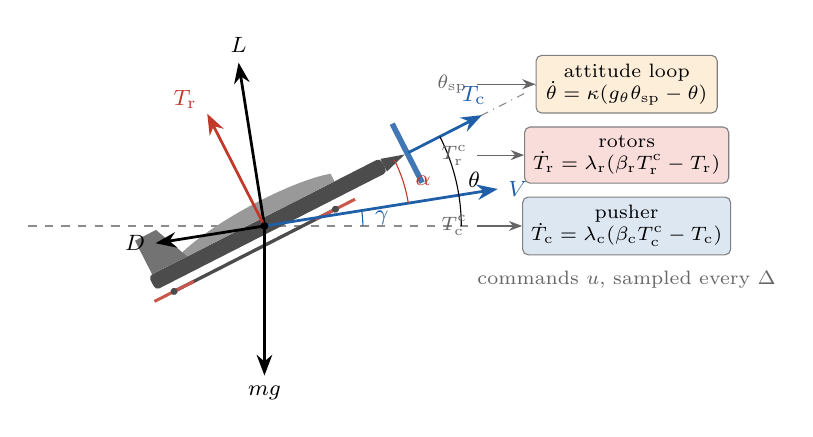
\begin{tikzpicture}[>=Stealth, font=\footnotesize]
\def\gam{9} \def\th{27}
\coordinate (O) at (0,0);
\draw[black!45, dashed] (-3.0,0) -- (3.6,0) node[right, black!60, font=\scriptsize] {horizon};
\draw[black!45, dash dot] (\th+180:1.6) -- (\th:3.7) node[right, black!60, font=\scriptsize] {body axis};
\begin{scope}[rotate=\th]
  \fill[black!70, rounded corners=1.5pt] (-1.6,-0.1) rectangle (1.7,0.1);
  \fill[black!70] (1.7,0.09) -- (2.0,0) -- (1.7,-0.09) -- cycle; \fill[csch!85] (2.0,-0.42) rectangle (2.07,0.42);
  \fill[black!40] (-1.1,0.1) -- (-1.1,0.17) .. controls (-0.55,0.34) and (0.55,0.36) .. (1.05,0.21) -- (1.05,0.1) -- cycle;
  \fill[black!55] (-1.55,0.1) -- (-1.55,0.58) -- (-1.25,0.58) -- (-1.05,0.1) -- cycle;
  \draw[black!70, line width=1.2pt] (-1.4,-0.22) -- (0.9,-0.22);
  \foreach \x in {-1.4,0.9}{\draw[cmpc!85, line width=1.1pt] (\x-0.28,-0.22) -- (\x+0.28,-0.22); \fill[black!70] (\x,-0.22) circle (0.045);}
\end{scope}
\draw[->, csch, line width=1pt] (O) -- (\gam:3.0) node[right, csch] {$V$};
\draw[->, line width=1pt] (O) -- (\gam+90:2.1) node[above] {$L$};
\draw[->, line width=1pt] (O) -- (\gam+180:1.4) node[left] {$D$};
\draw[->, csch, line width=1pt] (\th:2.05) -- (\th:3.1) node[above, csch, xshift=-3pt] {$T_{\mathrm c}$};
\draw[->, cmpc, line width=1pt] (O) -- (\th+90:1.6) node[above left, cmpc, yshift=-2pt] {$T_{\mathrm r}$};
\draw[->, line width=1pt] (O) -- (0,-1.9) node[below] {$mg$};
\fill[black] (O) circle (0.05);
\draw[csch] (1.25,0) arc (0:\gam:1.25) node[midway, right, xshift=1pt, csch] {$\gamma$};
\draw[cmpc] (\gam:1.85) arc (\gam:\th:1.85) node[midway, right, xshift=1pt, cmpc] {$\alpha$};
\draw (2.5,0) arc (0:\th:2.5) node[midway, right, xshift=1pt] {$\theta$};
% lag blocks
\begin{scope}[shift={(4.6,0.9)}]
\node[draw=black!50, rounded corners=2pt, fill=cphase!60, font=\scriptsize, minimum width=2.3cm, inner sep=3pt, align=center] (att) at (0,0.9) {attitude loop\\ $\dot\theta=\kappa(\gth\thsp-\theta)$};
\node[draw=black!50, rounded corners=2pt, fill=cband!60, font=\scriptsize, minimum width=2.3cm, inner sep=3pt, align=center] (rot) at (0,0.0) {rotors\\ $\dot T_{\mathrm r}=\lambda_{\mathrm r}(\beta_{\mathrm r}T^{\mathrm c}_{\mathrm r}-T_{\mathrm r})$};
\node[draw=black!50, rounded corners=2pt, fill=csch!15, font=\scriptsize, minimum width=2.3cm, inner sep=3pt, align=center] (pus) at (0,-0.9) {pusher\\ $\dot T_{\mathrm c}=\lambda_{\mathrm c}(\beta_{\mathrm c}T^{\mathrm c}_{\mathrm c}-T_{\mathrm c})$};
\draw[->, black!60] (-1.9,0.9) node[left, font=\scriptsize] {$\thsp$} -- (att.west); \draw[->, black!60] (-1.9,0.0) node[left, font=\scriptsize] {$T^{\mathrm c}_{\mathrm r}$} -- (rot.west); \draw[->, black!60] (-1.9,-0.9) node[left, font=\scriptsize] {$T^{\mathrm c}_{\mathrm c}$} -- (pus.west);
\node[font=\scriptsize, black!60, anchor=north] at (0,-1.35) {commands $u$, sampled every $\Delta$};
\end{scope}
\end{tikzpicture}
\end{document}
